\documentclass [9 pt]{article}
\usepackage[margin = 1in]{geometry}
\usepackage{amsfonts}
\usepackage{amsthm}
\usepackage{bbm}
\usepackage{amsmath}
\usepackage{arydshln}
\usepackage[utf8]{inputenc}
\usepackage{graphicx}
\usepackage{enumerate}
\usepackage{color}
\usepackage[dvipsnames]{xcolor}
\usepackage{graphicx}
\graphicspath{ {./images/} }
\usepackage{tikz}
\usepackage{xcolor}
\usepackage{listings}
\usepackage{color}
\usepackage{algorithm}
\usepackage{algpseudocode}

\definecolor{dkgreen}{rgb}{0,0.6,0}
\definecolor{gray}{rgb}{0.5,0.5,0.5}
\definecolor{mauve}{rgb}{0.58,0,0.82}


\lstset{
  language=Matlab,
  basicstyle=\ttfamily,               
  numbers=left,                  
  stepnumber=1,                  
  numbersep=5pt,                  
  backgroundcolor=\color{white}, 
  showspaces=false,              
  showstringspaces=false,        
  showtabs=false,                
  tabsize=2,                     
  captionpos=b,                  
  breaklines=true,               
  breakatwhitespace=true,         
  title=\lstname,
  numberstyle=\tiny\color{Black},
  keywordstyle=\color{BrickRed},
  commentstyle=\color{dkgreen},
  stringstyle=\color{mauve},  
}

\theoremstyle{definition}
\newtheorem{problem}{Problem}
\newtheorem{theorem}{Theorem}
\newtheorem*{corollary}{Corollary}
\newtheorem{proposition}[theorem]{Proposition}
\newtheorem{lemma}[theorem]{Lemma}
\newtheorem{conjecture}[theorem]{Conjecture}

\newtheorem{definition}[theorem]{Definition}
\newtheorem{remark}[theorem]{Remark}
\newtheorem{example}[theorem]{Example}


\usepackage{fancyhdr}
\pagestyle{fancy}
\lhead{Yuhao Wu \quad 260711365} 
\rhead{\bfseries COMP 350 Midterm Review 2}
\cfoot{\thepage}
\renewcommand{\headrulewidth}{0.4pt}
\renewcommand{\footrulewidth}{0.4pt}


\setlength{\parindent}{0pt}


\begin{document}
\section*{Approximation of $f'(x)$}

$$ f'(x) \approx \dfrac{f(x + h) - f(x)}{ h } $$
$$ f'(x) \approx \dfrac{f(x + h) - f(x - h)}{ 2h } $$
\newline
\newline
\newline
Pay attention to \textbf{Numerical Cancellation:}
when $h$ is small, $f(x + h) - f(x) \to 0$
Re-formula the formula to avoid numerical cancellation.

\newpage
\section*{Solve Linear System: $AX = b$}
\subsection*{GENP:}
\lstinputlisting{genpMyVersion.m}

For the \textbf{first Loop(Line 10):}\\\\
We will first consider the  \textbf{inner Loop(Line 11):}\\
in each iteration:
We have 1 division first\quad (\textbf{Line 12})\\
We have $(n - k)$ multiplication and $(n - k)$ minus , total $ 2(n -k)  $\quad  (\textbf{Line 13}) \\
We have 1 multiplication and 1 minus \quad (\textbf{Line 14})\\
Thus, we have 
$$\big(1 + 2(n -k) + 2\big)(n - k)  $$
Thus for the total loop, we have
$$ \sum_{k = 1}^{n - 1}\big(1 + 2(n -k) + 2\big)(n - k) \approx 2\sum_{k = 1}^{n - 1}(n - k)^2 = 2 \times \bigg(1^2 + 2^2 \ldots + (n-1)^2 \bigg) \approx \dfrac{2}{3} n^3   $$
\\
\\
\\
For the \textbf{second Loop(Line 24):}\\
in each iteration:
We have $(n - k)$ multiplication and $(n - k)$ minus + 1 division, total $ 2(n -k) + 1 $\\
Then for the total Loop, we have 
$$\sum_{k = 1}^{n - 1} 2(n -k) + 1  $$
























\newpage
\lstinputlisting{genpXW.m}

Take our Matrix to be $\begin{bmatrix}
	2 & 2 & 3\\
	4 & 5 & 6\\
	6 & 8 & 9
\end{bmatrix}$ \\
\\
\\
After \textbf{line 13}, we will get $\begin{bmatrix}
	2 & 2 & 3\\
	2 & 5 & 6\\
	3 & 8 & 9
\end{bmatrix}$, which means \textbf{line 13} changes both $A(1,2), A(1,3)$\\
\\
\\
After \textbf{line 14}, we will get $\begin{bmatrix}
	2 & 2 & 3\\
	2 & 1 & 0\\
	3 & 2 & 0
\end{bmatrix}$, which means \textbf{line 14} changes both $A(2,2), A(2,3), A(3,2) ,A(3,3)$\\
\\
I noticed in Matlab Debugger, it says $i = [2, 3]$ when I go into the loop.
Here $A(i,i)$ is the matrix  $A(k+1:n\  ,\ k+1:n)$ as $i = k+1:n$.\\
\\
When $k=1$, this is just $A(2:3\ ,\ 2:3)$.



















\newpage
\subsection*{GEPP:}
Question: Why we do partial pivoting?
\begin{itemize}
	\item GENP will fail $\implies$ as the first element may be 0, there could be cases that divide by 0
	\item avoid unnecessary loss of accuracy as $GENP$ is numerical stable
\end{itemize}
\lstinputlisting{geppMyVersion.m}
\textbf{COST}: Flop cost is the same as before $\dfrac{2}{3}n^3$ and we need  $\dfrac{1}{2}n^2$
\newpage
\lstinputlisting{geppXW.m}









\newpage
\section*{LU Factorization With Partial Pivoting}
\lstinputlisting{luppMyVersion.m}

\newpage
This is how we use LUPP to solve linear equations:
\\
\\
\lstinputlisting{luppSolve.m}





\newpage
\subsection*{Theoretical Results:}
Accuracy depends on
\begin{itemize}
	\item Algorithm
	\item Condition of Problems
\end{itemize}


\subsection*{Tridiagonal Matrix:}
Algorithm
\begin{itemize}
	\item In class, ideas are from $GENP$
	\item In midterm, you may be asked to write ideas from $GEPP$
\end{itemize}
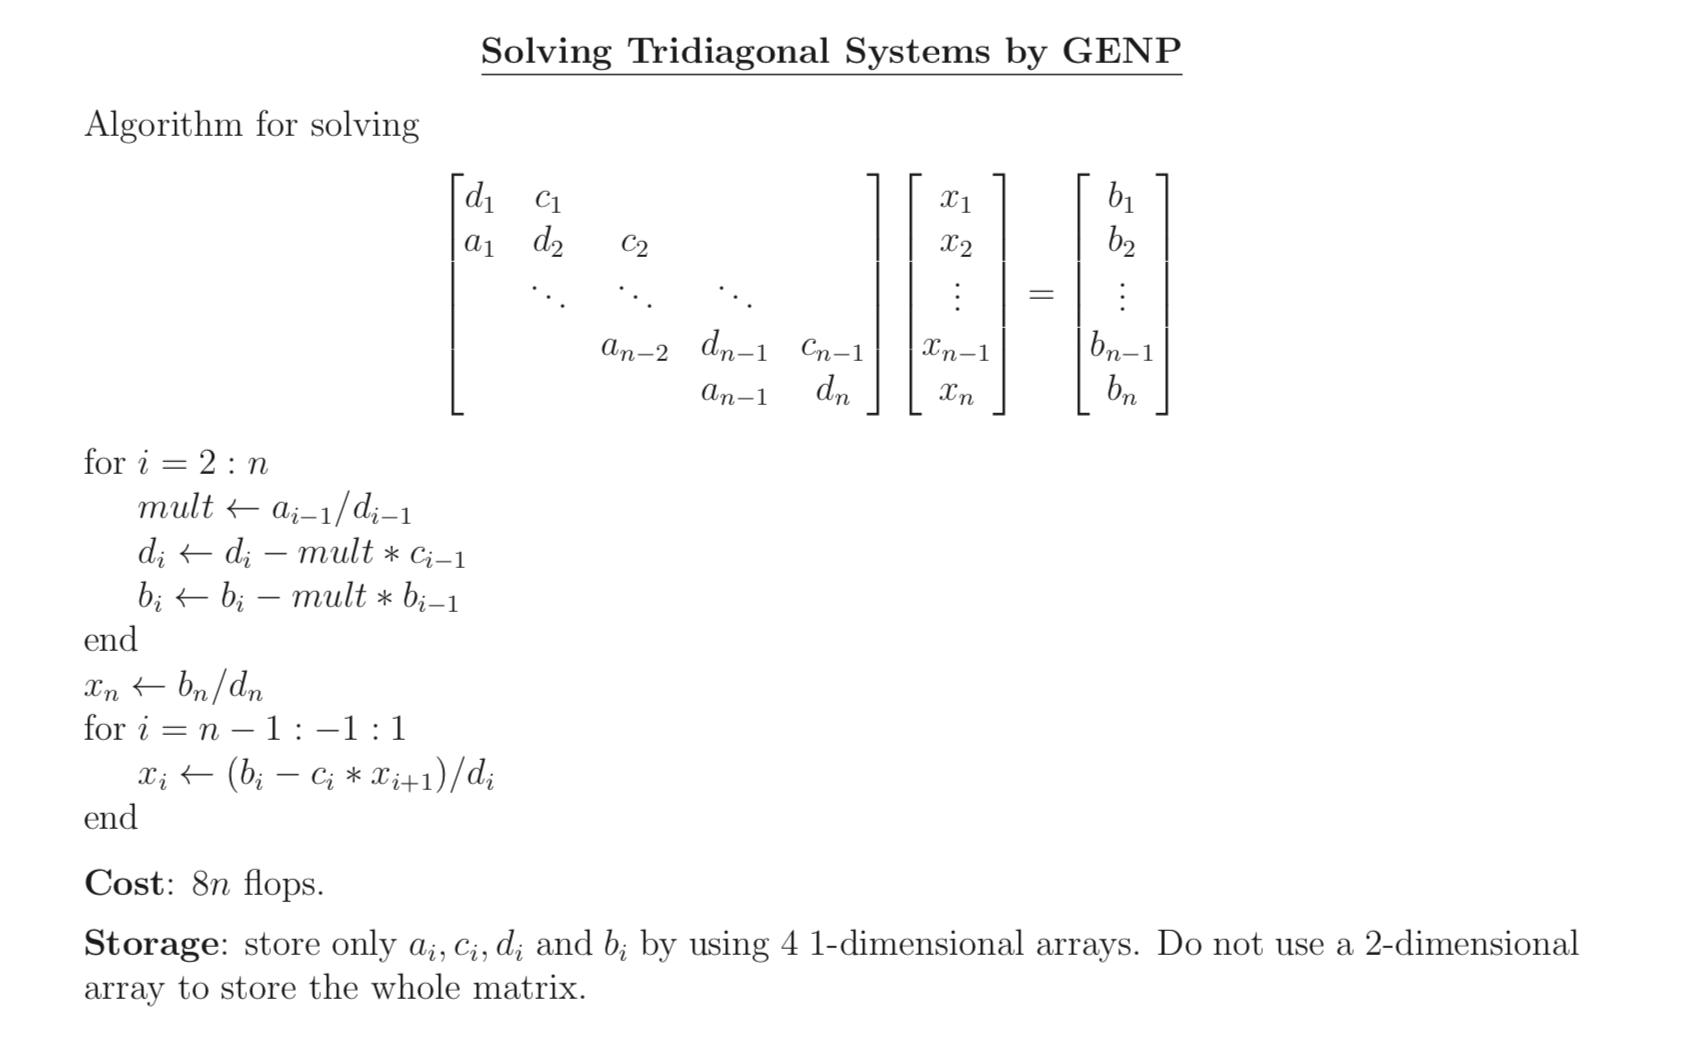
\includegraphics[scale = 0.5]{4.png}\\
\\
\section*{Diagonally Dominant Matrices}
Let $A = (a_{ij})_{n\times n}$. $A$ is strictly diagonally dominant by column if
$$ |a_{jj}| > \sum_{i = 1, i \neq j}^{n} |a_{ij}|\   for \ j = 1:n $$
\\
\\
Let $A = (a_{ij})_{n\times n}$. $A$ is strictly diagonally dominant by row if
$$ |a_{ii}| > \sum_{j = 1, i \neq j}^{n} |a_{ij}|\   for \ i = 1:n$$

\newpage
If a tridiagonal A is strictly diagonally dominant by column, then partial pivoting is not needed, i.e., GENP and GEPP will give the same results.
\\
\\
If $A$ is SDDC, then we have
\begin{itemize}
	\item $ |d_1| > |a_1|$
	\item $ |d_i| > |c_{i-1} | + |a_{i} |  $
	\item $ |d_n| > |c_{n - 1}|$
\end{itemize}
\textbf{Step 1:}\\
$multi = \dfrac{a_1}{d_1} < 1$; so there is no pivoting this step  \\\\
$d_2' =  d_2 - \dfrac{a_1}{d_1} \times c_1 $\\
So, we just need to show the matrix bounded by $d_2'$ is also SDDC.\\
Obviously, we just need to show $| d_2' | > |a_2| $\\
\begin{align*}
	| d_2' | 
	&=  |d_2 - \dfrac{a_1}{d_1} \times c_1 |\\
	&\geq |d_2| - |\dfrac{a_1}{d_1} \times c_1 |\\
	&\geq |d_2| - |\dfrac{a_1}{d_1}| \times | c_1 |\\
	&\geq |d_2| - | c_1 |\quad \quad as \ |d_2| > |a_2| + |c_1|  \\
	&> |a_2| 
\end{align*}
\\
\\
\newline
If a tridiagonal A is strictly diagonally dominant by row, then GENP will not fail
\\
If $A$ is SDDR, then we have
\begin{itemize}
	\item $ |d_1| > |c_1|$
	\item $ |d_i| > |a_{i-1} | + |c_{i} |  $
	\item $ |d_n| > |a_{n - 1}|$
\end{itemize}
\textbf{Step 1:}\\
Since $|d_1| > |c_1| \geq 0$, GENP won't fail in first step\\
\\
\textbf{Step 2:}\\
$d_2' =  d_2 - \dfrac{a_1}{d_1} \times c_1 $\\
So, we just need to show the matrix bounded by $d_2'$ is also SDDR.\\
Obviously, we just need to show $| d_2' | > |c_2| $\\
\begin{align*}
	| d_2' | 
	&=  |d_2 - \dfrac{a_1}{d_1} \times c_1 |\\
	&\geq |d_2| - |\dfrac{a_1}{d_1} \times c_1 |\\
	&\geq |d_2| - |\dfrac{c_1}{d_1} \times a_1 |\\
	&\geq |d_2| - |\dfrac{c_1}{d_1}| \times | a_1 |\\
	&\geq |d_2| - | a_1 |\quad \quad as \ |d_2| > |a_1| + |c_2|  \\
	&>|c_2| 
\end{align*}

\newpage
\section*{Using GEPP to solve Tridiagonal Matrix}
\renewcommand\arraystretch{1.5}
$$\begin{bmatrix}
	d_1 & c_1 & p_1 & 0 & 0 &0\\
	a_1 & d_2 & c_2 & p_2 & 0 &0\\
	0 & a_2 & d_3 & c_3 & p_3 &0\\
	0 & 0 & a_3 & d_4 & c_4 &p_4\\
	0 & 0 & 0 & a_4 & d_5 &c_5\\ 
	0 & 0 & 0 & 0 & a_5 &d_6\\ 	
\end{bmatrix} \times \begin{bmatrix}
	x_1\\
	x_2\\
	x_3\\
	x_4\\
	x_5\\
	x_6
\end{bmatrix} = \begin{bmatrix}
	b_1\\
	b_2\\
	b_3\\
	b_4\\
	b_5\\
	b_6
\end{bmatrix} $$
We will use 5 1-D array to store the matrix $d, c, a, p, b$\\
$P$ is initialized to 0 at the beginning, when we change two lines, there will be one more elements which will be stored to $p$
\begin{algorithm}
  \caption{Using GEPP to solve Tridiagonal Matrix}
  \begin{algorithmic}[1]
	\For{$i = 2 \to n - 1 $}
		\If{$|d_{i-1}| = |a_{i-1}| = 0$}
			\State "Error"
		\EndIf
		\If{$|d_{i-1}| < |a_{i-1}|$}
			\State $d_{i - 1} \Leftrightarrow a_{i - 1}$
			\State $d_{i } \Leftrightarrow c_{i - 1}$
			\State $p_{i - 1} \Leftrightarrow c_{i }$
			\State $b_{i } \Leftrightarrow b_{i - 1}$
		\EndIf
		\State $multi = \dfrac{a_{i-1}}{d_{i-1}}$\\
		\State $d_i = d_i - multi \times c_{i-1}$
		\State $c_i = c_i - multi \times p_{i-1}$
		\State $b_i = b_i - multi \times b_{i-1}$
	\EndFor\\
		\If{$|d_{n-1}| < |a_{n-1}|$}
			\State $d_{n - 1} \Leftrightarrow a_{n - 1}$
			\State $d_{n } \Leftrightarrow c_{n - 1}$
			\State $b_{n } \Leftrightarrow b_{n - 1}$
		\EndIf
		\State $multi = \dfrac{a_{n-1}}{d_{n-1}}$\\
		\State $d_n = d_n - multi \times c_{n-1}$
		\State $b_n = b_n - multi \times b_{n-1}$
\\	
	\State $x_n = \dfrac{b_n}{d_n}$
	\\
	\State $x_{n-1} = \dfrac{b_{n-1} - c_{n - 1 }\times x_n}{d_n}$
	\For{ $i = n - 2 \to -1$}
	\\
		\State $x_i = \dfrac{b_i - c_i \times x_{i+1} - p_i \times x_{i+2}}{d_i}$
	\\
	\EndFor
  \end{algorithmic}
\end{algorithm}



\end{document}